\documentclass[border=10pt]{standalone}

\usepackage{tikz}
\usepackage{tikzsymbols}
\usetikzlibrary{calc,patterns,shapes.geometric}

\def\centerarc[#1](#2)(#3:#4:#5){\draw[#1] ($(#2)+({#5*cos(#3)},{#5*sin(#3)})$) arc (#3:#4:#5);}

\begin{document}
	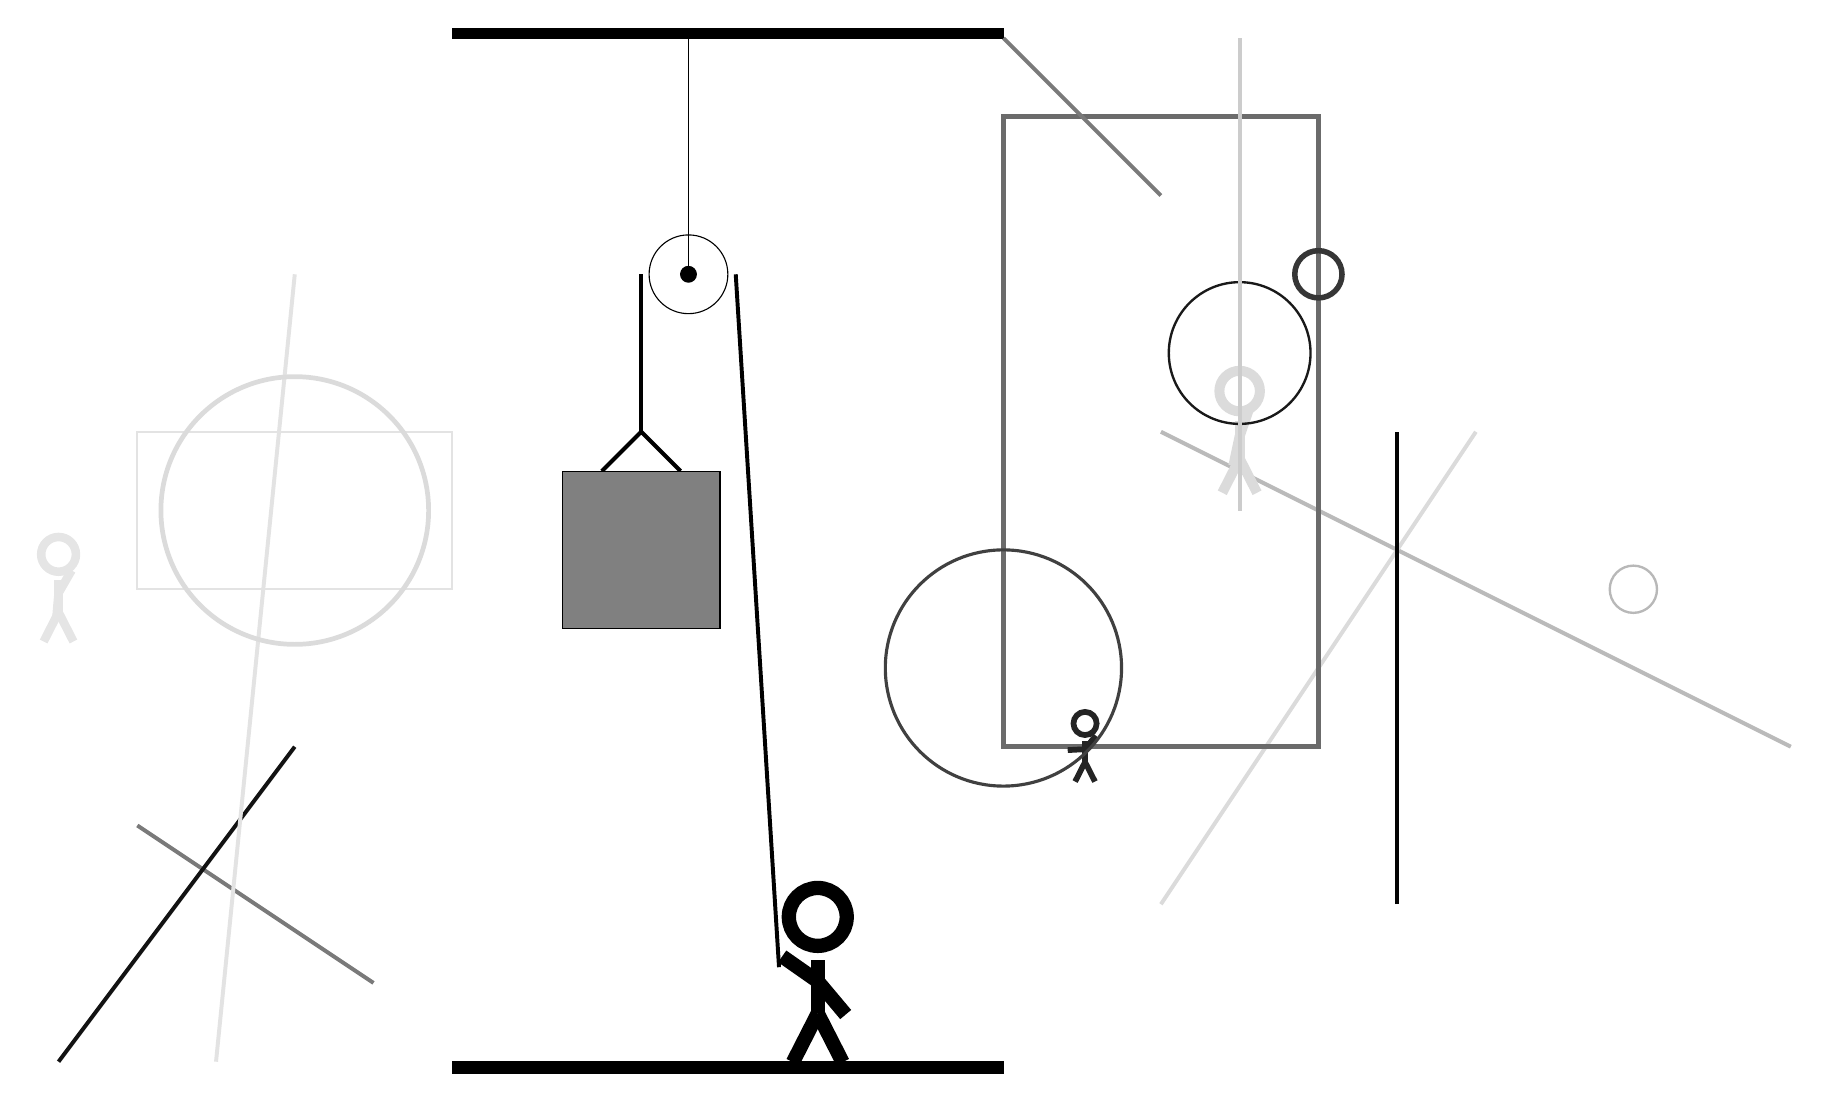
\begin{tikzpicture}
		%%%%% START %%%%%
		
		\draw[fill=black] (-2, 10) rectangle (5, 10.125);
		
		\draw (1, 7) circle (0.5);
		\draw[fill=black] (1, 7) circle (0.1);
		\draw (1, 10) -- (1, 7);
		
		\draw[line width=0.5mm] (-0.1, 4.5) -- (0.4, 5.0) -- (0.9, 4.5);
		\draw[fill=black!50] (-0.6, 4.5) rectangle (1.4, 2.5);
		
		\draw[line width=0.5mm] (0.4, 7) -- (0.4, 5.0);
		\centerarc[line width=0.5mm](1, 7)(0:180:0.6);
		\draw[line width=0.5mm](1.6, 7) -- (2.15, -1.8);
		
		\node at (2.6, -1.9) {\Strichmaxerl[10][-35][-50]};
		
		\draw[line width=0.5mm, color=black!27](7, 5) -- (15, 1);
		
		\draw[line width=0.5mm, color=black!14](7, -1) -- (11, 5);
		\node[line width=0.6mm, color=black!14] at (8, 5) {\Strichmaxerl[7][78][71]};
		\draw[line width=0.3mm, color=black!11] (-2, 3) rectangle (-6, 5);
		\draw [line width=0.3mm, color=black!28](13, 3) circle (0.3);
		
		\draw[line width=0.5mm, color=black!52](-6, 0) -- (-3, -2);
		\draw[line width=0.5mm, color=black!93](-7, -3) -- (-4, 1);
		\draw[line width=0.6mm, color=black!58] (5, 1) rectangle (9, 9);
		\draw [line width=0.3mm, color=black!90](8, 6) circle (0.9);
		\node[line width=0.5mm, color=black!86] at (6, 1) {\Strichmaxerl[4][3][52]};
		\node[line width=0.2mm, color=black!10] at (-7, 3) {\Strichmaxerl[6][85][60]};
		
		\draw [line width=0.4mm, color=black!75](5, 2) circle (1.5);
		\draw [line width=0.7mm, color=black!79](9, 7) circle (0.3);
		
		\draw[line width=0.5mm, color=black!20](8, 10) -- (8, 4);
		\draw[line width=0.5mm, color=black!52](5, 10) -- (7, 8);
		\draw[line width=0.5mm, color=black!11](-5, -3) -- (-4, 7);
		
		\draw [line width=0.6mm, color=black!14](-4, 4) circle (1.7);
		\draw[line width=0.5mm, color=black!99](10, -1) -- (10, 5);
		
		\draw[fill=black] (-2, -3) rectangle (5, -3.15);
		
		%%%%% END %%%%%
	\end{tikzpicture}
\end{document}